\documentclass[11pt]{article}
\usepackage{mypackages}
\begin{document}

\maketitle

\section{Introduction}

For human beings the natural way of learning is through repeatedly solving the same
task over and over again, each time observing the result and connecting
actions with outcomes.

In the context of machine learning, the same principles can be used to find the
sequence of actions that provide the best outcome for a given task
- a technique known as \textit{reinforcement learning}.
The goal of this project is to investigate the advantages of asynchronous reinforcement
learning in an advanced setting - playing Atari 2600 games\cite{openAIEnvs}.

Solving a task this way consists of being in a certain state and making a decision,
which leads to a new state with a new set of decisions to be made, until
a terminal state is reached.
The terminal state is reached when there are no more decisions to be made
and the task is finished.
Thus a task can be seen as a \textit{decision tree}, with actions connecting states to future states.
%%%%%% Task decision tree
\begin{figure}[H]
    \centering
    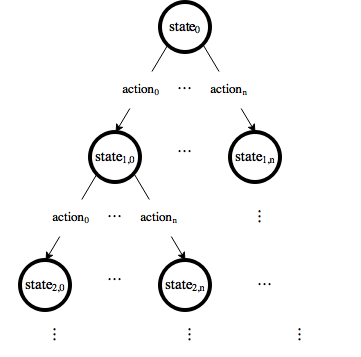
\includegraphics[scale=0.5]{include/decision_tree.png}
    \caption{A decision tree for solving a task.}
    \label{fig:dec_tree}
\end{figure}

In a typical reinforcement learning setting we try to solve a problem
by moving downwards through the decision tree until a terminal state is reached.
The result of taking this exact path is then
taken into account the next time the algorithm tries to solve the problem.

\subsection{Inspiration}

In December 2013 the DeepMind Technologies team published an article
describing an approach on how to learn from a high dimensional sensory input -
frames from an Atari environment -
using deep reinforcement learning\cite{dqn}.
With a combination of \textit{Convolutional Neural Networks} (CNN) and
the reinforcement learning method Q-learning\cite{RLbook} - an approach they
dubbed \textit{Deep Q-Networks} (DQN) - they
presented results proving that it was possible to learn how to play Atari
games, at a superhuman level, with the frames of the game as the only input.

Previous reinforcement learning methods haven't been able to succeed at learning to play
advanced games, but the combination of neural networks and
reinforcement learning have made it possible.

An emerging problem with learning to play advanced games, is the computational time and
resources it takes to train the algorithm.
Thus a general approach used to solve reinforcement learning problems is to
play through a game and continuously evaluate and update the way actions are picked
while playing the game.
Choosing the best actions depends on what state the player is in, but it is difficult to
know which action is best before every option is explored.
A solution to the resource problems of reinforcement learning,
is to play a game many times in parallel,
allowing multiple paths in the decision tree to be explored at the same time -
a method called \textit{asynchronous training}.

%As a way to lower the time of training the traditional reinforcement
%learning algorithm can be implemented to do asynchronous training.
%This way the algorithm can take advantage of modern GPUs since
%they are able to execute instructions in parallel\cite{gpu_stuff}.
%Learning asynchronously in this way seems straight forward in deep
%reinforcement learning, since deep neural networks can be optimised
%for GPU usage.

One way to train asynchronously is to run multiple instances of the same program
in a lot of threads on a single CPU.
Most modern CPUs consists of multiple cores, which means it is possible to have a thread
running on each core without interfering with each other.
Each thread can then use the experience of the other threads 
to evaluate and change its own strategy if another thread
has found a better one.

The team responsible for the Deep Q-Networks approach collaborated with
the Montreal Institute for Learning Algorithms (MILA) in June 2016 article
\cite{a3c} where multiple reinforcement learning methods were implemented to
take advantage of asynchronous training.

\subsection{Methods}

With the results of the Google DeepMind team in mind\cite{a3c}, the scope of the project we present in
this paper, will be to implement the \textit{Actor-Critic} algortihm according to \cite{RLbook}
with a deep learning approach, for learning how to play the simple game of \textit{Cart-Pole}\cite{cart_pole}
as a proof of concept.
We will then extend this idea to the \textit{Asynchronous Advantage Actor-Critic} (A3C)
method presented in \cite{a3c} and examine the effects of different amounts of threads
on the A3C algorithm as it learns to play the Cart-Pole problem and selected Atari games.

A3C is a reinforcement learning method that is able to learn
how to solve a problem solely from experience.
The algorithm uses two separate Convolutional Neural Networks
 - one to extract information about the algorithms performance 
and the other to select which action to perform.
These two networks can be seen as the body and the brain of a human.
The body performs actions which are evaluated by the brain and if
the action leads to a good result, the brain reinforces the idea
of repeating the action in the future, if it should ever be in a similar
situation.

We use CNN's since they have proved to work well on extracting features
of Atari frames in previous projects (\cite{dqn}, \cite{a3c}).
They are computationally expensive to update though,
so to decrease the amount of necessary computations we will limit
the input by preprocessing the frames before feeding them
to the networks, following the approach suggested in \cite{dqn-nature}.
In \cite{a3c} more than one optimization scheme
is suggested, but the focus in this project is on the effect of
different amounts of threads so we won't be tuning hyperparameters
and testing different optimization strategies.
Thus, this project will not focus on playing Atari games really well,
but instead on how asynchronous training affects the stability of
reinforcement learning methods.

In the remainder of this paper we review the 
Cart-Pole and Atari environments available to us in
the OpenAI Gym framework and examine the theory behind the
reinforcement and deep learning methods we will be using
- i.e. the Actor-Critic algorithm and the asynchronous strategy of A3C.
We will also provide the results of the Actor-Critic algorithm
on the Cart-Pole game compared to the A3C method, as well as the
results of the A3C algorithm playing Atari games, with different 
amounts of threads. 
Lastly the implementation and experimental setup will be presented and
a discussion of the results will be given as well as ideas for further
work.

%%%% Dette skal kun med hvis vi ikke kan gøre vores eget trådet
%However, due to the time limitations of the project, we will focus on
%the implementation of the Actor-Critic algorithm and only alter
%an already existing implementation of the a3c method.
%%%%

%In order to test the performance and stability of the Actor-Critic
%method, we will be using learning environments provided by OpenAI
%gym\cite{openAI} - an open source project which aims at providing
%a simple interface to a collection of reinforcement learning tasks.
%This collection contains a lot of Atari 2600 environments, which we will
%use to compare our results to those presented in \cite{a3c}.

%The main focus of this project is the stability of reinforcement learning
%tasks and how asynchronous learning can be used to achieve better
%stabiliyty.
%We will be presenting the results of the Actor-Critic method used on a
%simpler task than the Atari environments - the cartpole problem
%\cite{cart_pole} - and then compare an asynchronous approach to the
%results of the DQN-method\cite{dqn} as well as the a3c
%algorithm\cite{a3c}.

%In the remainder of the paper we present and review the reinforcement
%learning environments in the Open AI gym collection and examine the
%theory behind the reinforcement learning methods that will be used -
%i.e. the Actor-Critic algorithm.
%Furthermore, results of the Actor-Critic approach to solving the cart-pole
%problem as well as the comparison between our asynchronous approach and
%the one produced by the Google Deepmind team are given.
%Lastly a discussion of these results and the stability problem as a whole
%is presented as well as ideas for further work.

%\printbibliography
%\bibliography{citations}
%\bibliographystyle{plain}
\end{document}
